%\emph{•}%%%%%%%%%%%%%%%%%%%%%%%%%%%%%%%%%%%%%%%%%
% Short Sectioned Assignment
% LaTeX Template
% Version 1.0 (5/5/12)
%
% This template has been downloaded from:
% http://www.LaTeXTemplates.com
%
% Original author:
% Frits Wenneker (http://www.howtotex.com)
%
% License:
% CC BY-NC-SA 3.0 (http://creativecommons.org/licenses/by-nc-sa/3.0/)
%
%%%%%%%%%%%%%%%%%%%%%%%%%%%%%%%%%%%%%%%%%
%----------------------------------------------------------------------------------------
%	PACKAGES AND OTHER DOCUMENT CONFIGURATIONS
%----------------------------------------------------------------------------------------
\documentclass[norsk]{article} % A4 paper and 11pt font size

\usepackage[T1]{fontenc} % Use 8-bit encoding that has 256 glyphs
\usepackage{fourier} % Use the Adobe Utopia font for the document - comment this line to return to the LaTeX default
\usepackage[english]{babel} % English language/hyphenation
\usepackage{amsmath,amsfonts,amsthm} % Math packages

% Added by Haavard %---------------------------------------------------------------------
\usepackage[utf8]{inputenc} % Norwegian letters
\usepackage{fullpage}
\usepackage{subcaption}
\usepackage[font={small, it}]{caption} % captions on figures and tables
\usepackage{graphicx}
\usepackage{color}
\usepackage{hyperref} % Use \autoref{ and \nameref{
\hypersetup{backref,
  colorlinks=true,
  breaklinks=true,
  %hidelinks, %uncomment to make links black
  linkcolor=blue,
  urlcolor=blue,
  citecolor=blue
}
\usepackage[all]{hypcap} % Makes hyperref jup to top of pictures and tables
% --------------------------------------------------------------------------------------
% Added by Jorgen %--------------------------------------------------------------------
\usepackage{enumitem}
% Added by Jorgen, for source code listing %-------------------------------------------
\usepackage{wrapfig}

\usepackage{listings}
\usepackage{xcolor}
\newcommand{\textcolordummy}[2]{#2}

\definecolor{mygray}{rgb}{0.4,0.4,0.4}
%\definecolor{mycyan}{rgb}{0,0.8,0.6}
\definecolor{mygreen1}{rgb}{0.3,0.6,0.3}
\definecolor{mygreen2}{rgb}{0,0.4,0.1}
\definecolor{myorange}{rgb}{1.0,0.4,0}

\lstset{language=C++,
                basicstyle={\color{black}\footnotesize\ttfamily\let\textcolor\textcolordummy},
                %identifierstyle=\color{green},
                keywordstyle={\color{blue}\footnotesize\ttfamily\let\textcolor\textcolordummy},
                %keywordstyle={\color{blue}\footnotesize\ttfamily\let\textcolor\textcolordummy},
                directivestyle={\color{mygreen1}},
                emph={int,char,double,float,unsigned},
                emphstyle={\color{mygreen2}},
                %
                stringstyle={\color{myorange}\footnotesize\ttfamily\let\textcolor\textcolordummy},
                %stringstyle={\color{orange}\footnotesize\ttfamily\let\textcolor\textcolordummy},
                commentstyle={\color{mygray}\footnotesize\ttfamily\let\textcolor\textcolordummy},
                morecomment=[l][\color{magenta}]{\#}
                %
                showspaces=false,  
                showstringspaces=false, 
                showtabs=false,
                extendedchars=true,
                frame=single,  
}
\lstdefinestyle{FormattedNumber}{%
    literate={0}{{\textcolor{red}{0}}}{1}%
             {1}{{\textcolor{red}{1}}}{1}%
             {2}{{\textcolor{red}{2}}}{1}%
             {3}{{\textcolor{red}{3}}}{1}%
             {4}{{\textcolor{red}{4}}}{1}%
             {5}{{\textcolor{red}{5}}}{1}%
             {6}{{\textcolor{red}{6}}}{1}%
             {7}{{\textcolor{red}{7}}}{1}%
             {8}{{\textcolor{red}{8}}}{1}%
             {9}{{\textcolor{red}{9}}}{1}%
             {.0}{{\textcolor{red}{.0}}}{2}% Following is to ensure that only periods
             {.1}{{\textcolor{red}{.1}}}{2}% followed by a digit are changed.
             {.2}{{\textcolor{red}{.2}}}{2}%
             {.3}{{\textcolor{red}{.3}}}{2}%
             {.4}{{\textcolor{red}{.4}}}{2}%
             {.5}{{\textcolor{red}{.5}}}{2}%
             {.6}{{\textcolor{red}{.6}}}{2}%
             {.7}{{\textcolor{red}{.7}}}{2}%
             {.8}{{\textcolor{red}{.8}}}{2}%
             {.9}{{\textcolor{red}{.9}}}{2}%
             ,
   basicstyle=\footnotesize\ttfamily,%  Optional to use this
}

%---------------------------------------------------------------------

\usepackage{lipsum} % Used for inserting dummy 'Lorem ipsum' text into the template

\usepackage{sectsty} % Allows customizing section commands
\allsectionsfont{\centering \normalfont\scshape} % Make all sections centered, the default font and small caps

\usepackage{fancyhdr} % Custom headers and footers
\pagestyle{fancyplain} % Makes all pages in the document conform to the custom headers and footers
\fancyhead{} % No page header - if you want one, create it in the same way as the footers below
\fancyfoot[L]{} % Empty left footer
\fancyfoot[C]{} % Empty center footer
\fancyfoot[R]{\thepage} % Page numbering for right footer
\renewcommand{\headrulewidth}{0pt} % Remove header underlines
\renewcommand{\footrulewidth}{0pt} % Remove footer underlines
\setlength{\headheight}{13.6pt} % Customize the height of the header

\numberwithin{equation}{section} % Number equations within sections (i.e. 1.1, 1.2, 2.1, 2.2 instead of 1, 2, 3, 4)
\numberwithin{figure}{section} % Number figures within sections (i.e. 1.1, 1.2, 2.1, 2.2 instead of 1, 2, 3, 4)
\numberwithin{table}{section} % Number tables within sections (i.e. 1.1, 1.2, 2.1, 2.2 instead of 1, 2, 3, 4)

\setlength\parindent{0pt} % Removes all indentation from paragraphs - comment this line for an assignment with lots of text

%----------------------------------------------------------------------------------------
%	TITLE SECTION
%----------------------------------------------------------------------------------------

\newcommand{\horrule}[1]{\rule{\linewidth}{#1}} % Create horizontal rule command with 1 argument of height

%\title{	
%\normalfont \normalsize 
%\textsc{NTNU} \\ [25pt] % Your university, school and/or department name(s)
%\horrule{0.5pt} \\[0.4cm] % Thin top horizontal rule
%\huge C++  Notes \\ % The assignment title
%\horrule{2pt} \\[0.5cm] % Thick bottom horizontal rule
%}

%\author{Jørgen Vågan} % Your name

%\date{\normalsize\today} % Today's date or a custom date

\begin{document} %---------------------------------------

%\maketitle % Print the title

%\section{Spørsmål Runde 1 }
%Jeg har funnet et program kalt \textbf{Engauge Digitizer} til å lese av grafene. Sliter litt med 
%at den ikke identifiserer alle kurvene og sliter med overlappende biter.
%\newline
%\begin{wrapfigure}{r}{0.6\textwidth} %Requires the package wrapfigure
  %\begin{center}
    %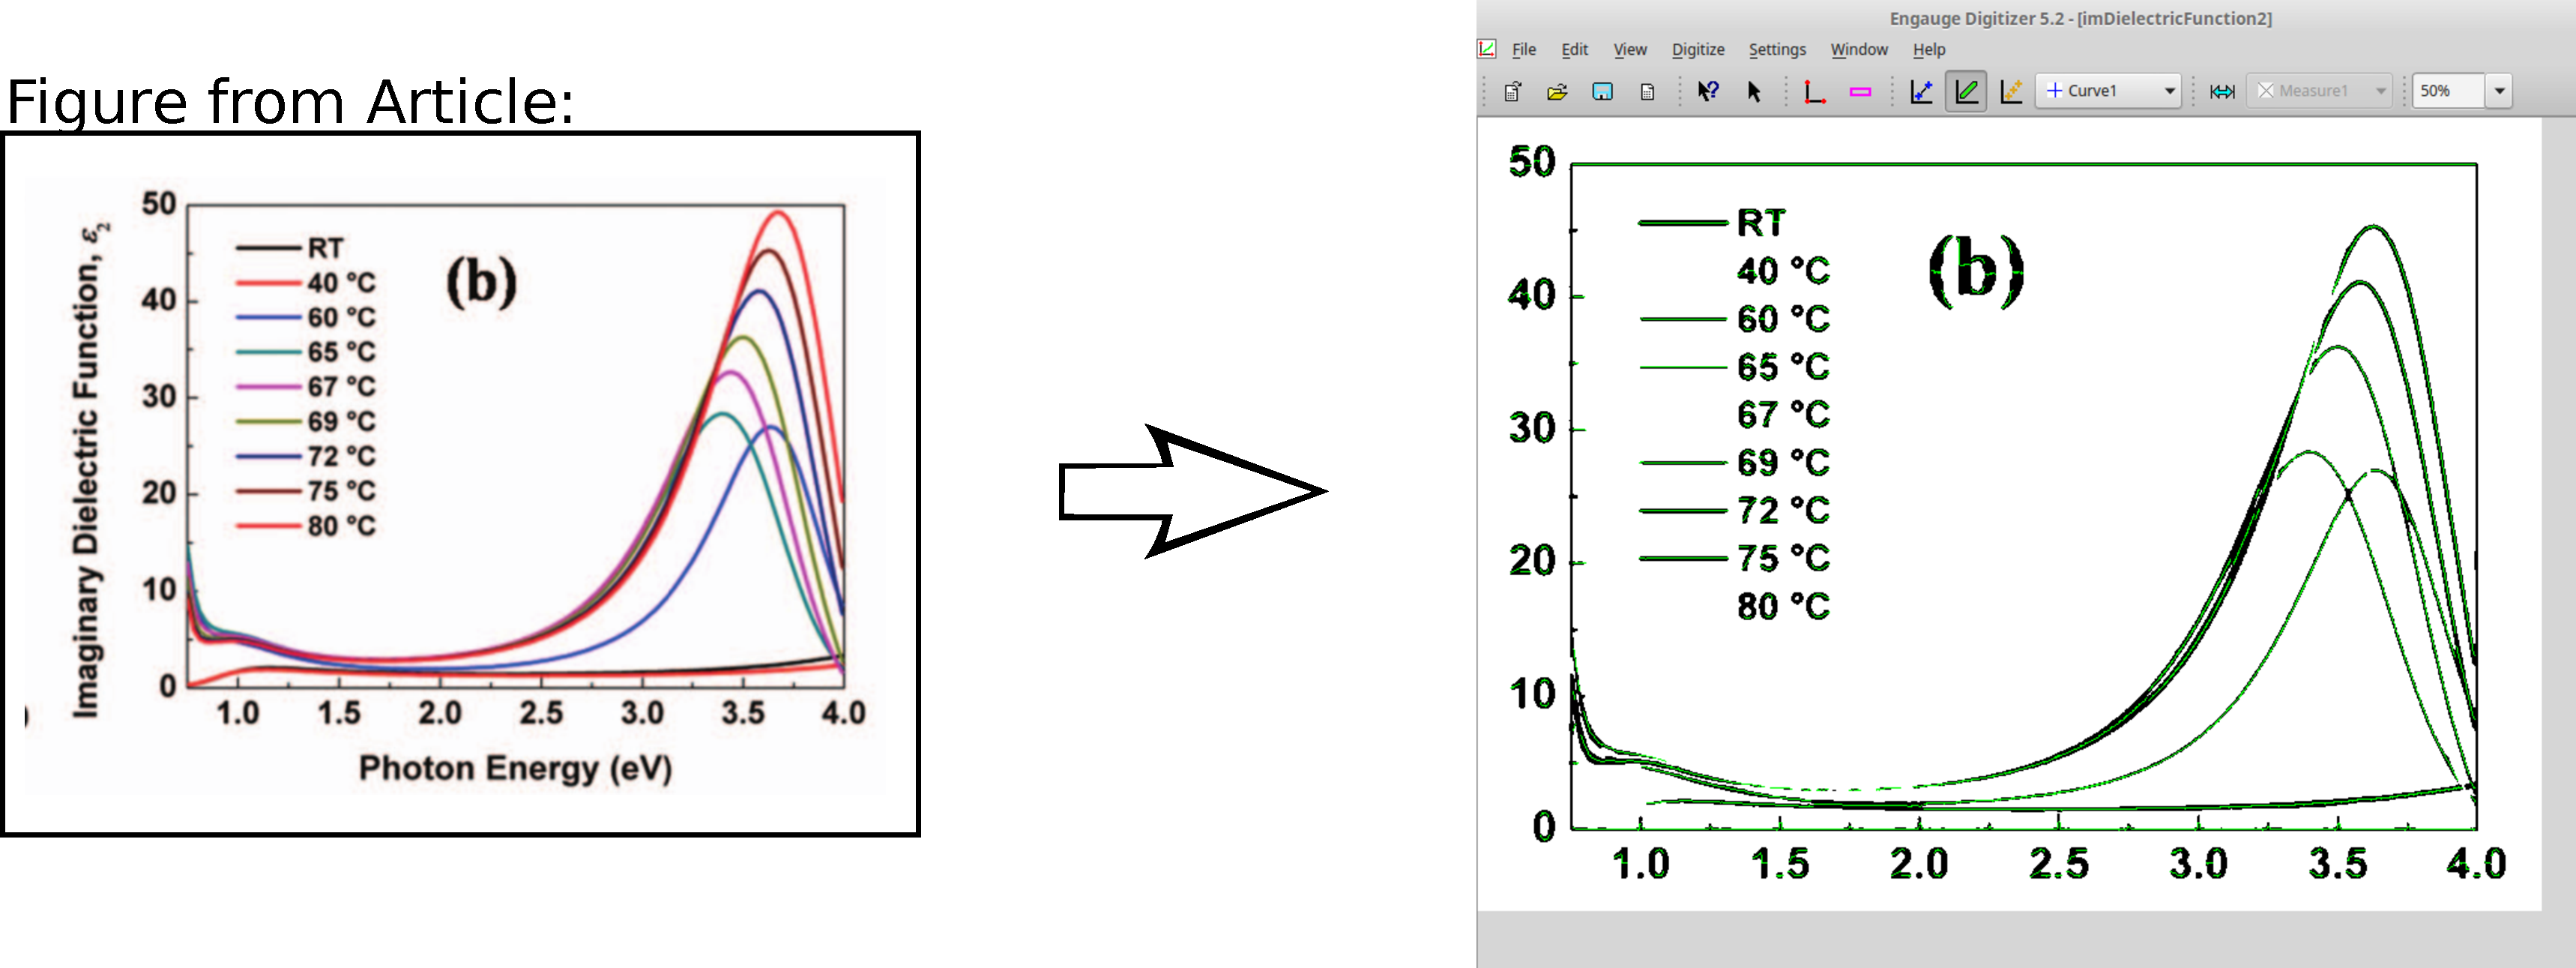
\includegraphics[width=0.58\textwidth]{engaugeExample.pdf}
  %\end{center}
%\end{wrapfigure}
Jeg prøver å forstå mer detaljert hvordan jeg skal få lest inn dataen til GranFilm programmet.
Formatet til ''.nk''-filene i \texttt{GranFilm/Sopra/DataBase} ser slik ut (her mgo.nk):
\begin{lstlisting}[style=FormattedNumber,frame=none]
   1		0.65			10		400    
        1.70969699     0.00000011
        1.71065583     0.00000011
        1.71239613     0.00000011
\end{lstlisting}
og ser ut til å ha reell og imaginær refraksjonsindeks forholdsvis på kolonne 1 og 2. I tillegg virker det
som om rad èn består av de 4 verdiene: 
\begin{itemize}
   \item unit (om refraksjonsindeksen er funksjon av energi (eV) 
eller bølgelengde); 
\item x startverdi (energi/bølgelengde); 
\item x sluttverdi
\item antall datapunkter.
\end{itemize}
Basert på dette, i tillegg til modulen fra source-koden til GranFilm gitt nedenfor, virker det
som om reell og imaginær verdi er gitt for samme x-verdi (energi/bølgelengde), der x-verdiene 
har konstant steglengde. (For eksempel: for mgo.nk filen ville vi hatt $d\!x = \frac{10-0.65}{400-1}$).
\\
\\
Jeg har funnet et program som lar meg hente ut dataen fra grafer i artikklene. 
Prolemet er at dataen for reell og imaginær refraksjonsindeks 
er for forskjellige x-verdier, der x-verdiene ikke har
konstant steglengde.\\
\\
\textbf{Spørsmålene er derfor:} 
\begin{enumerate}
   \item Er det riktig det jeg har forstått ovenfor? 
   \item Trenger jeg skrive om inputfilene (filene med thermochrom-dataen) 
      slik at reell og imaginær verdi (forholdsvis $n$,$k$)
      svarer til samme x-verdi, der x-verdiene ligger med avstand $d\!x$ i fra hverandre?\\
      (Jeg tenkte å kanskje skrive en funksjon som tar inn to filer, colonner og ''unit''-verdi, 
      leser inn $n$ og $k$ dataen fra filene, intrapolerer for felles, nye x-verdier og skriver til 
      en ny fil.)
   \item Videre: noen grafer er gitt ved permittivitet $\varepsilon$, istedenfor refraksjonsindex \textbf{n}.
      Da er det vel bare å regne om ved bruk av imaginær permittivitet? Jeg fant noen formlet og lurte på 
      om dette er riktig: fant at 
      \begin{align*}
         \boldsymbol{\varepsilon} =
            \frac{c^2 \varepsilon_0}{\omega^2 \frac{\mu}{mu_0}} \Bigg( k^2 - \frac{\alpha ^2}{4}\Bigg)  
            + i\Bigg( \frac{c^2 \varepsilon_0}{\omega^2 \frac{\mu}{\mu_0}} k \alpha \Bigg)
      \end{align*}
      ($k$ er hær bølgetallet), hvor 
      \begin{align*}
         &\boldsymbol{n} = k - i\frac{\alpha}{2}, & \boldsymbol{n} = \frac{c}{\omega} \boldsymbol{k}^*.
      \end{align*}
      Bruker at $\mu = \mu_0$ og får
      \begin{align*}
         &\text{Re}(n) = \frac{\text{Im}(\varepsilon)}{2 \varepsilon_0} \\
         &\text{Im}(n) = \sqrt{\frac{\text{Re}(\varepsilon)}{\varepsilon_0} - 
         \Bigg( \frac{\text{Im}(\varepsilon)}{2 \varepsilon_0} \Bigg) ^2}.
      \end{align*}
\end{enumerate}

Til slutt vil jeg bare si at framgangen går sakte, og begynner å bli litt stresset mtp tiden. Lurte
på hvor mye du hadde forestilt deg at jeg burde få til? Foreløpig, har jeg klart å lese ut 
VO$_2$-dataen fra de fire artiklene du sendte meg. Dataene trenger trolig mer arbeid før de mates inn
i GranFilm som beskrevet ovenfor. Der ligger VO$_2$ data for 10-12 forskjellige temperaturer.


%I kildekoden til \texttt{GranFilm} fant jeg \texttt{dielectric\_function\_module.f90}:
%\begin{lstlisting}[style=FormattedNumber,frame=none, language=FORTRAN]
    %Read(unit=ifile,fmt=*) unit,x1,x2,lines
    %dx = (x2 - x1)/(lines-1)

    %Allocate( x(lines), y(lines) )
    %Select Case (unit)
    %Case(1)
       %! Unit = Electron Volt (eV)
       %Do i=1,lines 
          %Read(unit=ifile,fmt=*) tmp(1), tmp(2)
          %x(i) = x1 + (i-1)*dx
          %y(i) = tmp(1)+imu*tmp(2)
       %Enddo
    %Case(2)
       %! Unit = WaveLength (microm)
       %Do i=lines,1,-1 
          %Read(unit=ifile,fmt=*) tmp(1), tmp(2)
          %x(i) = x1 + (lines-i)*dx
          %y(i) = tmp(1)+imu*tmp(2)
       %Enddo
       %x(:) = 1.243\_wp/x(:) ! Conversion microm-->eV
    %End Select

    %Close(unit=ifile)
%\end{lstlisting}
%først leses første linje av \texttt{'.nk'}-filen:
%som gir \texttt{unit} (som er hva?), start energi/bølgelengde, slutt energi/bølgelengde og til slutt 
%antall datapunkter. Når du nå regner ut \texttt{x} og \texttt{y} virker det som om du antar at
%n,k-verdiene er gitt from samme energi(eV) eller bølgelengde. I tillegg virker det som at datapunktene
%må være separert med konstant steglengde $dx$. Men, i mine avleste data
%er ikke dette tilfellet: dataen er gitt for ulike verdier og steglengden varierer: 
%\begin{lstlisting}[style=FormattedNumber,frame=none]
   %//#! Fra fil reIndexOfRefractionVO2.csv,
   %x,n06,n13
   %3.40909e-07,1.96538,1.01971
   %3.45455e-07,2.12453,1.15231
   %3.61364e-07,2.68154,1.61639
   %.           .       .
   %.           .       .
%\end{lstlisting}
%\begin{lstlisting}[style=FormattedNumber,frame=none]
   %//#! Fra fil imIndexOfRefractionVO2.csv
   %x,k06,k13
   %3.41541e-07,1.44393,0.928804
   %3.42121e-07,1.43807,0.933948
   %3.51121e-07,1.34701,1.01382
   %.           .       .
   %.           .       .
%\end{lstlisting}
%Må jeg passe på at input-data-filen er slik som jeg har tolket ovenfor, altså:
%to kolonner (første med reel refraksjonsindex og andre med imaginer refraksjonsindex)
%der verdiene i en gitt rad er gitt for samme x-verdi (energi/bølgelengde)?\\
%\\
%Hele koden for funksjonen er hær:
I kildekoden til \texttt{GranFilm} \: fant jeg modulen \: \texttt{dielectric\_function\_module.f90}.
Forstår det slik at 
\begin{lstlisting}[style=FormattedNumber, language=FORTRAN, frame=none]
    Function Locate(xx,x)
\end{lstlisting}
finner indeksen i xx til elementet som ligger nærmest verdien x? Tenkte å kunne bruke
funksjonen eller skrive den om, og bruke den i intrapolering om jeg må skrive om input-filene.
\begin{lstlisting}[style=FormattedNumber, language=FORTRAN]
  !------------------------------------------------------------!
  Subroutine Get_Dielectric_Function(energy,epsilon,material,path)
  !Subroutine dielectric_constants(energy,epsilon,material,path)
  !------------------------------------------------------------!
    Use SFL_Logical_Units,       only : SFL_Get_Free_Unit
    Use Error_Module,            only : Error_Failure
    Implicit None
    Real(wp)                          :: energy(:)
    complex(wp )                      :: Epsilon(:)
    Character(len=*)                  :: material
    Character(len=*)                  :: path
    ! --- Local
    Character(len=*), parameter       :: routine = "Get_Dielectric_Function"
    !complex(wp ),Parameter            :: im=(0._wp,1._wp)
    Character(len=250)                :: filename, str
    Logical                           :: exi
    integer                           :: lines,start,i, ifile
    Real(wp),     Allocatable         :: x(:)
    complex(wp ), Allocatable         :: y(:)
    Real(wp)                          :: tmp(2),x1,x2,dx
    integer                           :: unit, istat
    complex(wp )                      :: slope
    

    ! Opens the relevant data file for the given material
    ! Notice that the data-files contains the values for the 
    ! index of refraction, n,k extacted from the data base of
    ! SOPRA.
    ! Therefore "epsilon = epsilon**2" at the bottom of this routine    
    filename = Trim(Adjustl(path))//'/'//Trim(Adjustl(material))//'.nk'
    Inquire(file=Trim(Adjustl(filename)),exist = exi)
    If( .NOT. exi ) Then
       write(str,*) trim(adjustl(filename))
       str = "File = " // trim(adjustl(str)) // " non existing" 
       Call Error_Failure(routine, trim(adjustl(str)) )
    Endif
    call SFL_Get_Free_Unit( ifile )
    Open(unit=ifile,file=filename,status='old')
    Read(unit=ifile,fmt=*) unit,x1,x2,lines
    dx = (x2 - x1)/(lines-1)

    Allocate( x(lines), y(lines) )
    Select Case (unit)
    Case(1)
       ! Unit = Electron Volt (eV)
       Do i=1,lines 
          Read(unit=ifile,fmt=*) tmp(1), tmp(2)
          x(i) = x1 + (i-1)*dx
          y(i) = tmp(1)+imu*tmp(2)
       Enddo
    Case(2)
       ! Unit = WaveLength (microm)
       Do i=lines,1,-1 
          Read(unit=ifile,fmt=*) tmp(1), tmp(2)
          x(i) = x1 + (lines-i)*dx
          y(i) = tmp(1)+imu*tmp(2)
       Enddo
       x(:) = 1.243_wp/x(:) ! Conversion microm-->eV
    End Select

    Close(unit=ifile)

    ! --- Do the interpolation
    Do i=1,Size(energy,1)
       start=locate(x(:),energy(i))
       If((start==0).Or.(start==lines)) Then
          write(str,"('Energy not in range : ',f5.2,' for i=',i3)") energy(i),i
          call Error_Failure( routine, trim(adjustl(str)))
       Endif
       ! Linear interpolation
       slope = (y(start+1)-y(start))/(x(start+1)-x(start))
       Epsilon(i) = y(start) + slope*(energy(i)-x(start))
       !            Write(unit=67,*) energy(i),Real(epsilon(i)),Aimag(epsilon(i))
    Enddo
    
    ! --- Calculates the dielectric constant (from the refraction index)
    epsilon = epsilon**2
    Deallocate(x,y,stat=istat)

  contains
    
    Function Locate(xx,x)
      Implicit None
      Real(wp), Dimension(:), Intent(In)  :: xx
      Real(wp), Intent(In)                :: x
      Integer                             :: locate
      Integer                             :: n,jl,jm,ju
      Logical                             :: ascnd
      
      n=Size(xx)
      ascnd = (xx(n) >= xx(1))
      jl=0
      ju=n+1
      Do
         If(ju-jl <= 1) exit
         jm=(ju+jl)/2
         If(ascnd .eqv. (x >= xx(jm))) Then
            jl=jm
         Else
            ju=jm
         Endif
      Enddo
      If(x == xx(1)) Then
         locate=1
      Else If(x == xx(n)) Then
         locate=n-1
      Else
         locate=jl
      Endif
      
    End Function Locate
    

  End Subroutine Get_Dielectric_Function
  !-------------------------------------!
\end{lstlisting}


%\section{Spørsmål Runde 2 }
Programmet som jeg bruker til å lese av grafene \textbf{Engauge Digitizer}.  
Lagde en kjapp oversikt før jeg startet. Bare legger den med, hvis du ikke er interessert er det bare å ignorere 
denne seksjonen:
\subsection{Engauge Digitizer, General Steps}
\textbf{Typical Steps:}
\begin{enumerate}
   \item Obtain image file (bmp, jpeg or other) showing one or more curves and both axes;
   \item Import image file using either:
      \begin{itemize}
         \item File/Import menu option;
         \item Copy-Paste;
         \item Drag and drop;
      \end{itemize}
   \item If important parts of the image is missing (e.g. parts of- or entire curves) or 
      curves are too thick (difficult to separate them),
      then go to \texttt{Settings/Discretize} and experiment with the discretization options
      until all curves are there and looking as nice as possible.
   \item Click on \texttt{Axes Point} button. 
   \item Click on click on one of the axes and enter graph coordinates.\\
         Repeat until you've added all axes (''origin'', point on x-axis and point on y-axis);
   \item Digitize graph: Click on the \texttt{Segment Fill} button to automatically digitize entire curve
         segments at a time or Click on the \texttt{Point Match} button to automatically digitize many 
         curve points. Click on a sample point and use the arrow keys to accept or reject points that match
      the sample point.


   \item Click on the \texttt{Curve Points} button to manually enter curve points by 
      clicking on the curve. Repeat until the curve is covered with a sufficient number of curve points.
   \item Export curve points by using either: 
      \begin{itemize}
         \item File/Export menu option to save selected curves into a tabular text file, or
         \item copy-pase / drag-drop points in the current curve from mthe \texttt{curve geometry window}
               to another application.
         \item Copy-Paste;
         \item Drag and drop;
      \end{itemize}
\end{enumerate}
Hær er et lite bilde av hvordan det importerte bildet set ut i engauge:
\begin{wrapfigure}{r}{0.6\textwidth} %Requires the package wrapfigure
  \begin{center}
    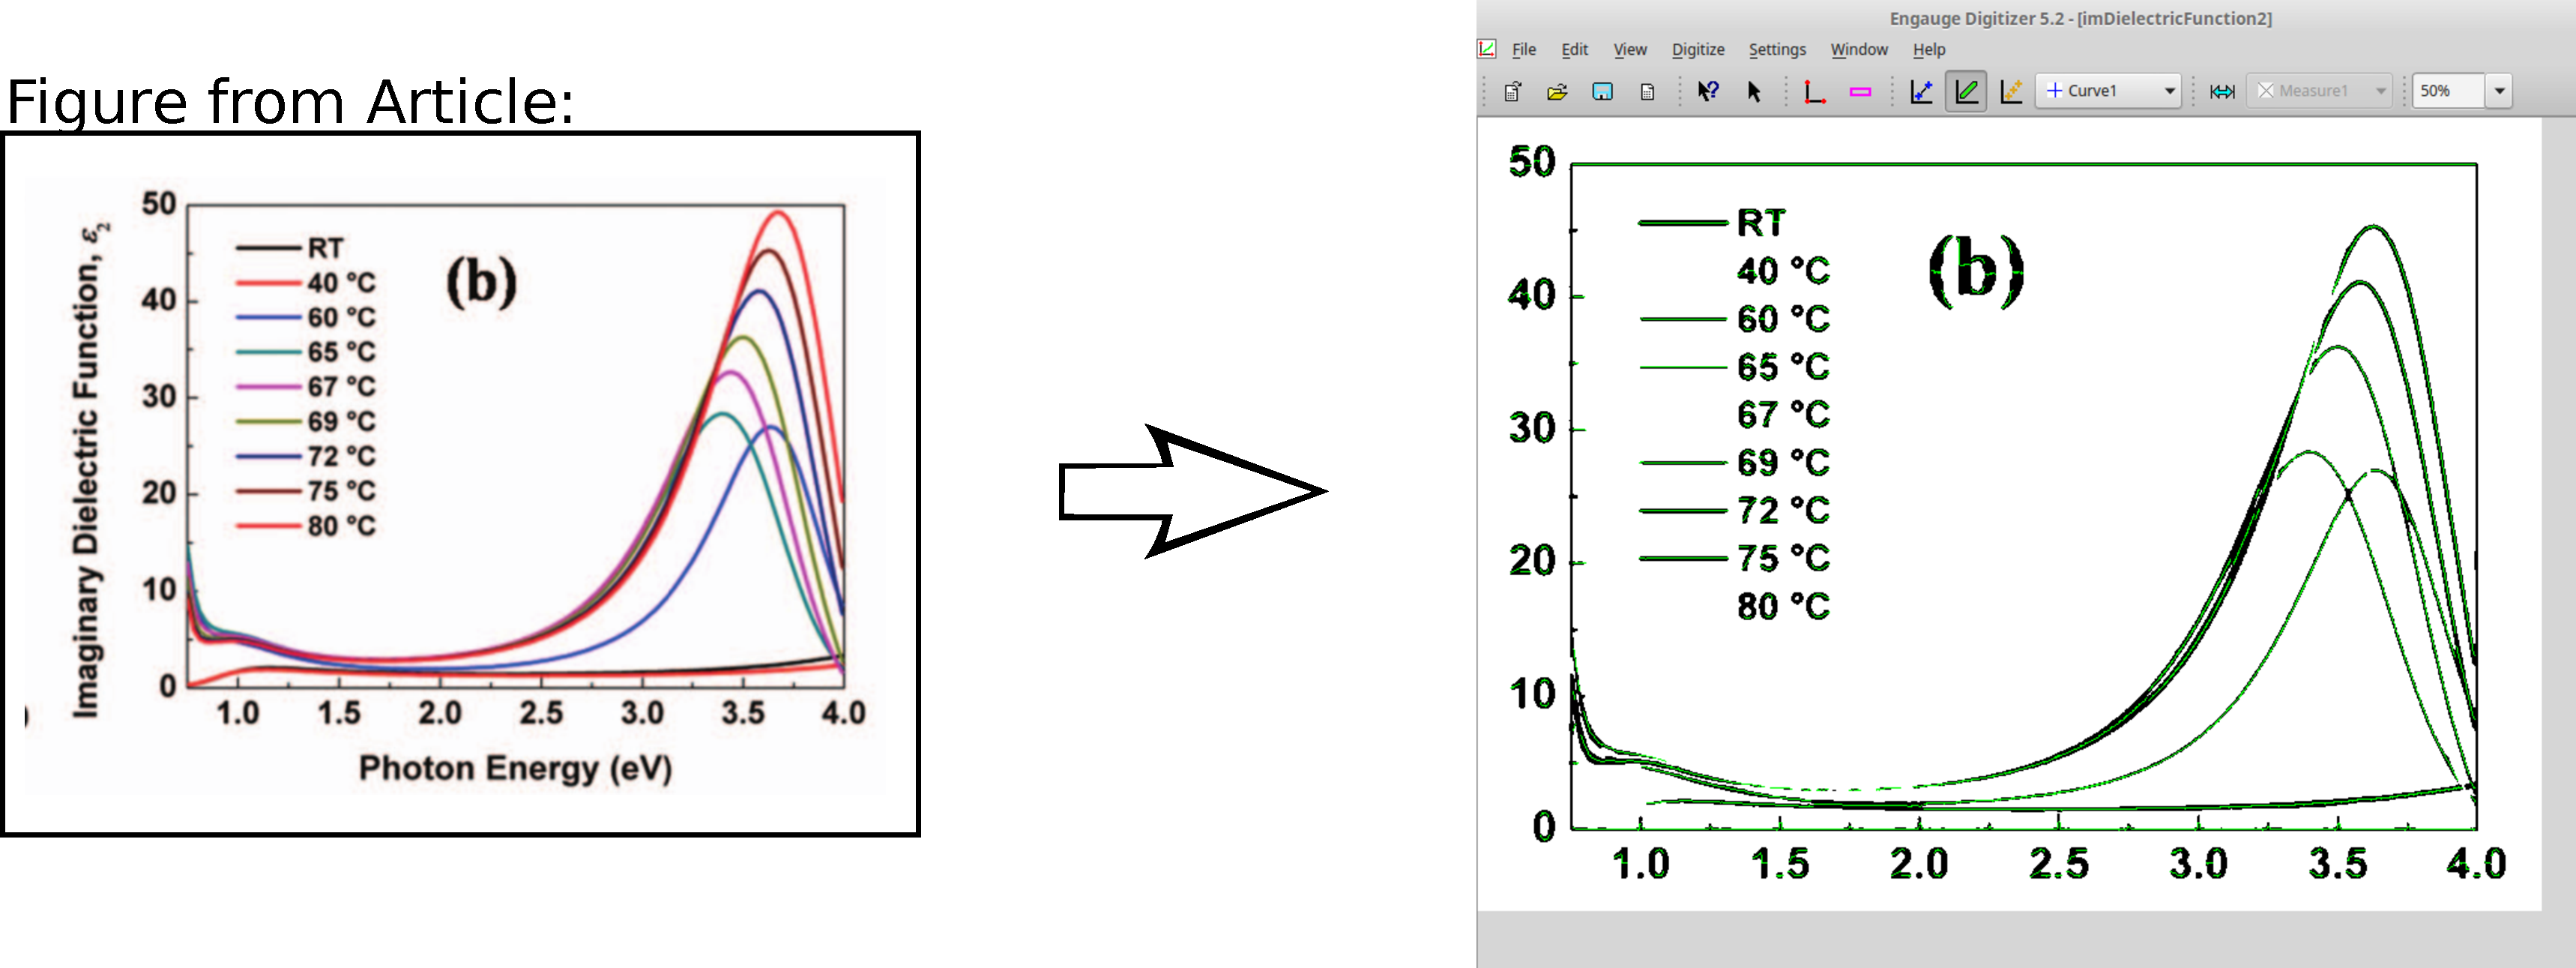
\includegraphics[width=0.58\textwidth]{engaugeExample.pdf}
  \end{center}
\end{wrapfigure}
%

\newpage
\subsection{Får ikke til å bruke scipy.interpolate funksjonene}
Jeg har prøvd å ekvidistansere datapunktene mine og intrapolere ved å bruke 
scipy.interp1d og scipy.griddata. Problemet er at jeg vil bare intrapolere
verdiene for det intervallet av x-verdiene der dataen for n- og k-verdiene overlapper.
Dette gjør at jeg ikke kan bruke de ovenfornevnte funksjonene, siden dimensjonene på
arrayene ikke stemmer. Hær er koden jeg har prøvd å bruke:
\newline
\begin{lstlisting}[style=FormattedNumber,frame=none, language=python]
#!/usr/bin/python
import numpy
#from scipy.interpolate import interp1d 
from scipy.interpolate import griddata

def find_nearest(array,value):
    i = (numpy.abs(array-value)).argmin()
    return i

#Of the largest min-values in the two arrays, this functions finds the index in the other array
# corresponding to this value:
def find_min_x(x1, x2): 
    if( x1[0] < x2[0] ):
        imin = find_nearest(x1, x2[0])
        if( x1[imin] < x2[0] ):
            imin = imin + 1
            return x1[imin]
        else: 
            return x2[0]
    else:
        imin = find_nearest(x2, x1[0])
        if( x2[imin] < x1[0]):
            imin = imin + 1
            return x2[imin]
        else:
            return x1[0]


def find_max_x(x1, x2): 
    if( x1[-1] < x2[-1] ):
        imax = find_nearest(x2, x1[-1])
        if( x1[-1] < x2[imax] ):
            imax = imax - 1
            return x2[imax]
        else: 
            return x1[-1]
    else:
        imax = find_nearest(x1, x2[-1])
        if( x2[-1] < x1[imax] ):
            imax = imax - 1
            return x1[imax]
        else: 
            return x2[-1]

\end{lstlisting}
%
\newpage
\begin{figure}[h!] 
\centering 
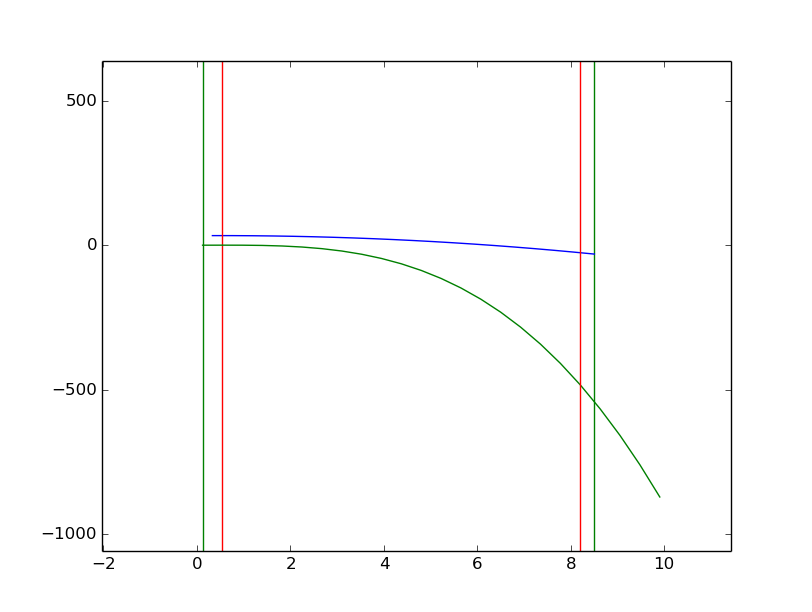
\includegraphics[width=0.5\textwidth]{dataBoundaries.png} 
\caption{Jeg bruker find\_nearest(), find\_min\_x() and find\_max\_x() for å finne hvor datapunktene 
overlapper og tar den første og siste verdien innenfor dette området. Disse verdiene brukes som
start og slutt verdi for energi/bølgelengde og vil bli skrevet ut i første linje av ''.nk'' filen. 
Denne grafen er bare en test for å se at funksjonene virker.} 
\end{figure}

Koden fortsetter:
\begin{lstlisting}[style=formattednumber,frame=none, language=python]
skipRows = 1 #input for numpy.loadtxt(). Skips the first row with the top information
valueDelimiter = ',' # input for numpy.loadtxt(). Tells which symbol that separates the data


unit = 2 #OUTPUT-LINE-1, x = wavelength
nData = numpy.loadtxt('reOpticalIndexVO2.csv', skiprows=skipRows, delimiter=valueDelimiter)
kData = numpy.loadtxt('imOpticalIndexVO2.csv', skiprows=skipRows, delimiter=valueDelimiter)

# Find lowest x-value which are in both datasets:
x1 = find_min_x(nData[0], kData[0])

# Find largest -value which are in both datasets:
x2 = find_max_x(nData[0], kData[0])

#Not sure about the number of data points so I just use the lowest of the two:
dataPoints = 150 #OUTPUT-LINE-1

firstLine = str(unit)+'\t'+str(x1)+'\t'+str(x2)+'\t'+str(dataPoints)  

# Interpolate the data such that we get the n,k values for the same equidistant x-values:
x = numpy.linspace(x1,x2, num=dataPoints, endpoint=True) #equidistant x-values
#try 1:
#n = interp1d(x,nData[:,1])
#k = interp1d(x,kData[:,1])
#try 2:
#n = griddata(nData[:,0], nData[:,1], x, method='linear')
#k = griddata(kData[:,0], kData[:,1], x, method='linear')

#write to file
numpy.savetxt('savetxtOutput.nk', numpy.column_stack((n,k)), delimiter='\t', header=firstLine, comments='')
#comments='' because if not, then the header would be a comment and contain the #-symbol
\end{lstlisting}

Feilmeldingene jeg får for å bruke interp1d() er: 
\begin{lstlisting}[style=formattednumber,frame=none, language=bash]
Traceback (most recent call last):
  File "./convertData.py", line 105, in <module>
      n = interp1d(x,nData[:,1])
  File "/usr/lib/python2.7/dist-packages/scipy/interpolate/interpolate.py", line 333, in __init__
      _Interpolator1D.__init__(self, x, y, axis=axis)
  File "/usr/lib/python2.7/dist-packages/scipy/interpolate/polyint.py", line 35, in __init__
      self._set_yi(yi, xi=xi, axis=axis)
  File "/usr/lib/python2.7/dist-packages/scipy/interpolate/polyint.py", line 94, in _set_yi
      raise ValueError("x and y arrays must be equal in length along "
ValueError: x and y arrays must be equal in length along interpolation axis.
\end{lstlisting}

Bruker jeg griddata() får jeg ingen feilmeldinger, men outputfilen min ser slik ut:
\begin{lstlisting}[style=formattednumber,frame=none, language=bash]
2	0.0607533	2.23613	150
nan	nan
nan	nan
nan	nan
nan	nan
nan	nan
nan	nan
nan	nan
nan	nan
nan	nan
nan	nan
\end{lstlisting}
Det er åpenbart at jeg prøver å gjøre noe som ikke er lov i første tilfellet og i andre tilfellet 
har jeg kanskje misforstått helt. Tenkte bare å høre om det jeg har startet å gjøre 
er fornuftig og om du hadde noen tips til hvordan jeg kan gå frem videre? Hvordan jeg evt.
kan løse problemet eller gå rundt det.

%\section{Spørsmål; Runde 3}
\begin{itemize}
   \item \textbf{Plasmoner og Overflate-Plasmoner}
      \begin{enumerate}
         \item Er størrelsene for ''polarizabilities'' $\alpha_{\parallel}$ og $\alpha_{\perp}$
            direkte relatert til plasmoner?
         \item Blir både bulk- og overflate-plasmoner eksitert i/på den granulære overflaten?
         \item Hvis ja, hvordan avviker den granulære overflaten fra en flat, glatt overflate
            mtp. plasmoner. \\
            Leste noe om at ujevnheter i overflaten ville føre til at overflate-plasmoner
            vil sende ut EM-stråling. Vil noe slikt føre til økt refleksjon av den inkommende bølgen?
      \end{enumerate}

   \item \textbf{"The coice of the reference Fresnel surface"/ "choice of the separation surface"}\\
      Dette blir nevnt under diskusjonen av "surface susceptibilities": $\delta, \tau, \gamma \beta$
      i GranFilm-artikkelen til deg og Lazzari på s.126 (siste avsnitt).
      Det står også at Fresnel størrelsene vil ikke endre seg mtp. valg av Fresnel overflate.
      Jeg forstår det slik at dette bare dreier seg om valg av referansesystem, altså 
      om man velger at den fysiske overflaten er satt $z=0$ eller en eller annen 
      $z=z_1 \neq 0$. Er dette riktig?
\end{itemize}


%\section{Spørsmål; Runde 4}
%Jeg har ikke helt evnene til å sette meg inn i all teorien som ligger bak GranFilm. Kan 
%i beste tilfellet bare satse på å tilegne meg en overfladisk forståelse. Dette vil mest sannsynligvis 
%vises i hvordan jeg har skrevet teorien, I og med at den er veldig knyttet til GranFilm-artikkelen og 
%masteroppgaven til Leif Amund Lie. Har prøvd å sette meg inn i teorien etter beste evne, og håper 
%jeg har formulert meg godt nokk med egne ord, selv om strukturen beklageligvis er den samme.
\begin{enumerate}[label=\textbf{\arabic*})]
   \item \textbf{Weak formulation of boundary conditions}\\
      \textbf{Hva er weak formulation of boundary conditions?} Utdrag fra artikkel:\\
      ''The usual way to treat the surface of the sphere is to use the orthogonality of the spherical 
      harmonics $Y_l^m(\theta,\phi)$ as functions of the ($\theta,\phi$) angles. This method, called weak
      formulation of the boundary conditions, leads to two infinite linear systems for the multipolar 
      coefficients $A_{lm}, B_{lm}$ for $m = 0, \pm 1$''

   \item \textbf{Sammenhengen mellom de første "multipole coefficients" $A_{lm}$, for $m = 0,\pm 1$,
      og ''polarizability''-størrelsene $\alpha$} er ikke helt klar, og virker ganske grunnleggende 
      for forståelsen av teorien. Er det noen enkel måte å forklare dette på? 

   \item Har nettopp laget et relativt generisk program \textsc{convertData.py} for å konvertere dataen 
      jeg får ut gjennom \textsc{Engauge Digitizer} fra artiklene (programmet ligger vedlagt for helheten,
      men må advare at det er veldig rotete, siden jeg ikke har brukt tid på å definere funksjoner).\\
      Uansett, jeg har inkludert muligheten til å konvertere fra permittivitet til "refraktive index"
      $\hat{n} = n + i\kappa$. Forrige gang var fremgangen min feil, så vil bare være sikker: \\
      \textbf{Er følgende konvertering fra $\hat{\varepsilon} \rightarrow \hat{n}$ riktig?:} \\
      \\
      The relative complex electric permittivity:
      \begin{align}
         \hat{\varepsilon}_r(\omega) = \frac{\hat{\varepsilon} (\omega)}{\varepsilon_0}
      \end{align}
      where 
      \begin{align}
         \hat{\varepsilon}_r(\omega) &= \varepsilon_r (\omega) + i\tilde{\varepsilon}_r (\omega) \\
                                     &= \varepsilon_r (\omega) + i\frac{\sigma}{\omega\varepsilon_0} 
      \end{align}
      The complex refractive index $\hat{n}$ is given by 
      \begin{align}
         \hat{n} = \sqrt{\hat{\varepsilon}_r},
      \end{align}
      when the magnetic properties are neglected ($\mu_r = 1$). 
      From this, an expression for the complex refractive index $\hat{n} = n + \boldsymbol{i}\kappa$ can be found:
      \begin{align}
         \hat{\varepsilon}_r &= \hat{n}^2 \\
         \varepsilon_r + \boldsymbol{i}\tilde{\varepsilon}_r &= (n + \boldsymbol{i} \kappa)^2 \\
         \varepsilon_r + \boldsymbol{i}\tilde{\varepsilon}_r &= n^2 - \kappa^2 + \boldsymbol{i}2n\kappa
      \end{align}
      giving
      \begin{align}
         \varepsilon_r &= n^2 - \kappa^2     &\tilde{\varepsilon}_r  &= 2n\kappa.
      \end{align}
      Taking the absolute value or modulus of the relative permettivity
      \begin{align}
         |\hat{\varepsilon}_r| &= \sqrt{ \varepsilon_r^2 + \tilde{\varepsilon}_r^2} \\
         |\hat{\varepsilon}_r| &= \sqrt{ (n^2 - \kappa^2)^2 + (2n\kappa)^2} \\
         |\hat{\varepsilon}_r|^2 &= (n^4 - 2n^2\kappa^2 + \kappa^4) + 4n^2\kappa^2 \\
         |\hat{\varepsilon}_r|^2 &= n^4 + 2n^2\kappa^2 + \kappa^4 \\
         |\hat{\varepsilon}_r|^2 &= (n^2 + \kappa^2)^2 \\
         |\hat{\varepsilon}_r| &= n^2 + \kappa^2 
      \end{align}
      and adding or substracting the real part of the permittivity, gives
      \begin{align}
         |\hat{\varepsilon}_r| + \varepsilon_r &= (n^2 + \kappa^2) + (n^2 - \kappa^2) = 2n^2\\
         |\hat{\varepsilon}_r| - \varepsilon_r &= (n^2 + \kappa^2) - (n^2 - \kappa^2) = 2\kappa^2.
      \end{align}
      Refomulating the expression gives the real and imaginary parts of $\hat{n}$
      \begin{align}
         n      &= \sqrt{ \frac{|\hat{\varepsilon}_r| + \varepsilon_r}{2}} 
                 = \sqrt{ \frac{|\hat{\varepsilon}| + \varepsilon}{2\varepsilon_0}}\\
         \kappa &= \sqrt{ \frac{|\hat{\varepsilon}_r| - \varepsilon_r}{2}} 
                 = \sqrt{ \frac{|\hat{\varepsilon}| - \varepsilon}{2\varepsilon_0}}
      \end{align}
      \textbf{Dette har jeg implementert på følgende måte:} 
      \begin{lstlisting}[style=FormattedNumber, language=python]
# (...)
re = re_interpolator(x) #interpolated equidistanced REAL values
im = im_interpolator(x) #interpolated equidistanced IMAGINARY values

#---------------------------------------------------------------------------------
# If the input data is given as permittivity/dielectric function, 
# we have to convert to the refractive index given by n,k:
if( isPermittivity ):
    import scipy.constants
    epsilon0 = scipy.constants.epsilon_0 

    # convert from permittivity to refractive index n and absorbtion coeff k:
    absEpsilon = numpy.sqrt( re**2 + im**2)
    n = numpy.sqrt( (absEpsilon + re)/2.0*epsilon0 )
    k = numpy.sqrt( (absEpsilon - re)/2.0*epsilon0 )

else: # the real data should be n, and the imaginary data should be k:
    n = re
    k = im
#---------------------------------------------------------------------------------
# (...)
     \end{lstlisting}
      \textbf{Ser dette riktig ut?} 


   \item 
      Klarte å få ut noen resultater for "half-infinite"-VO$_2$ ved 300$^{\circ}$K i luft/vacuum
      (plottet kjapt i xmgrace figur \ref{fig1}, \ref{fig2}, \ref{fig3}, beklager manglende infromasjon om
      kurvene). 
      \textbf{Slik som jeg har vinklet oppgaven
      min, hadde det vært interessant å finne ut hvordan materialet hadde oppført seg som 
      en tynn film på et materiale med ca. samme optiske egenskaper som glass. Har du noen
   forslag til noen slike materialer?} (Jeg må sjekke om noe slik data overlapper med den 
   visuelle/infraføde regionen, slik at det kan brukes som substrat).
      \begin{figure}[h!] 
      \centering 
      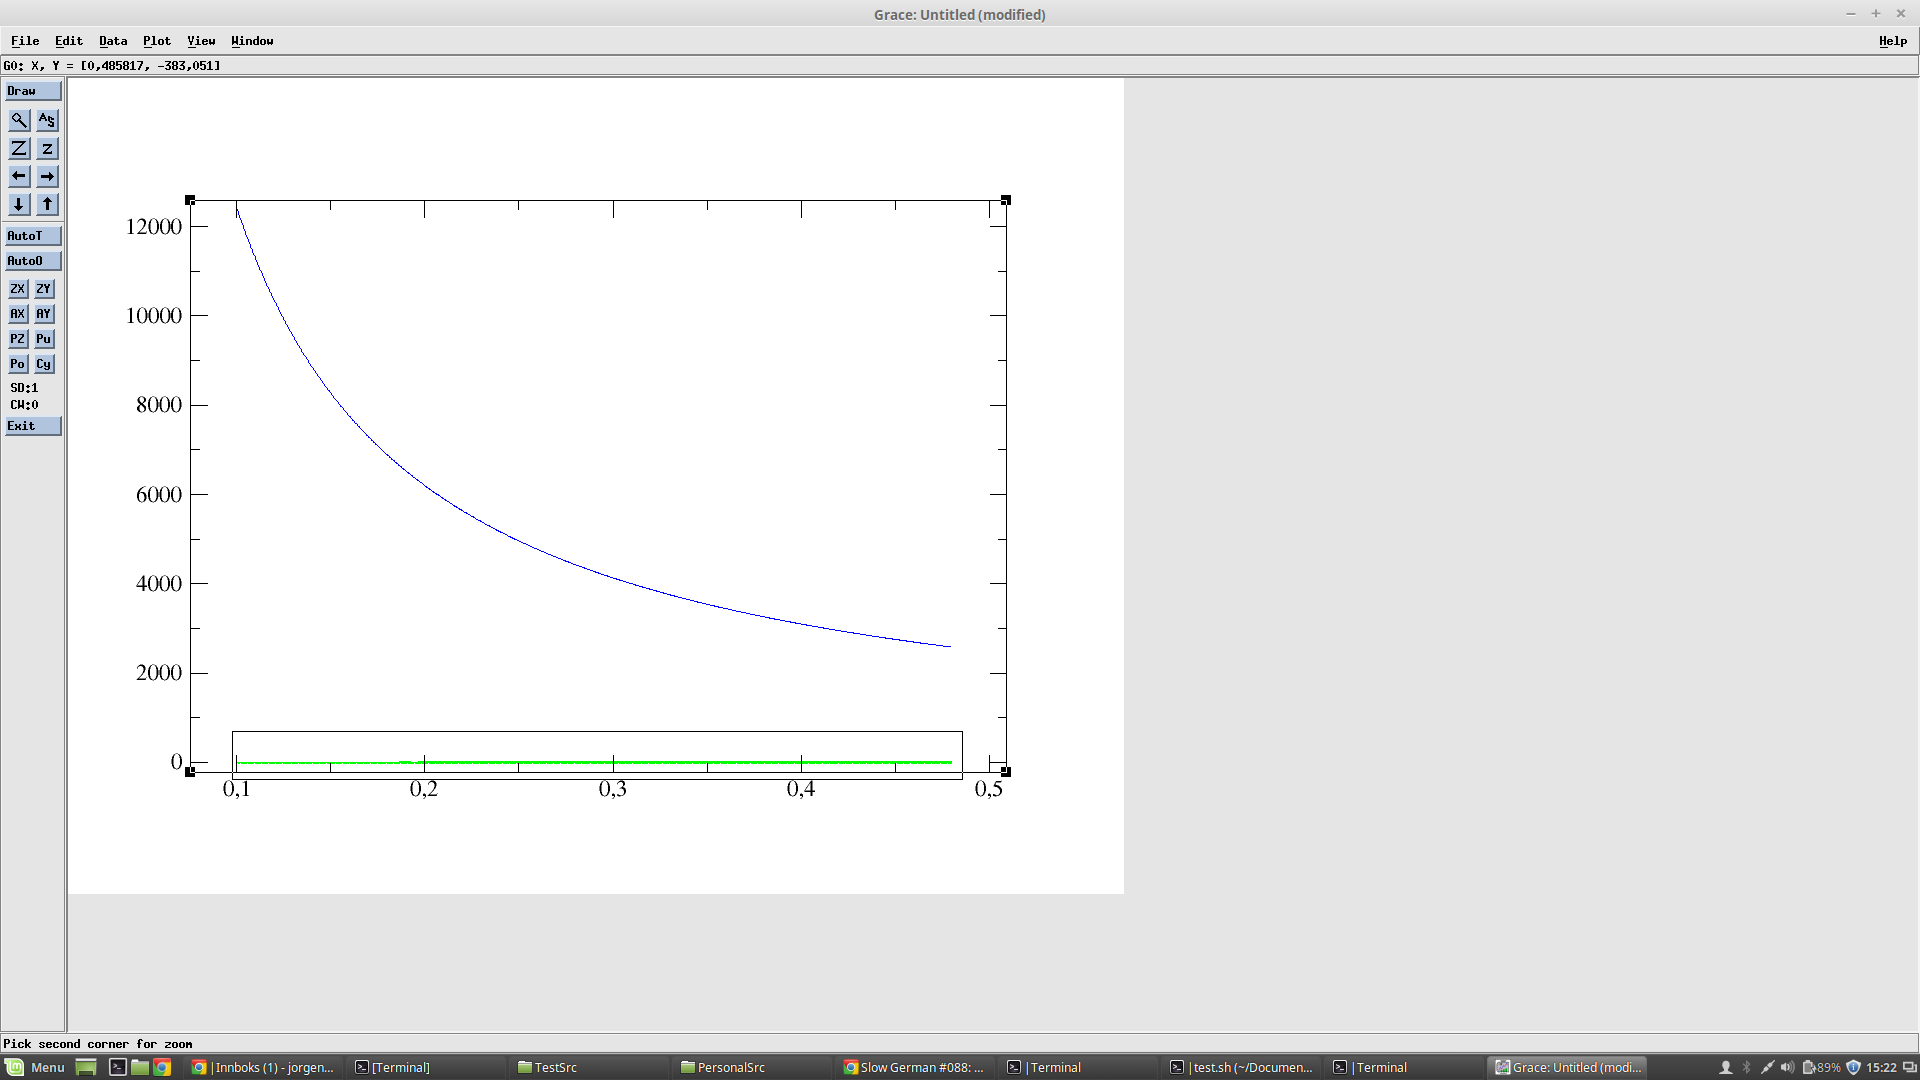
\includegraphics[width=1.0\textwidth]{Figures/result1a.png} 
      \caption{}
      \label{fig1}
      \end{figure}
      %
      \begin{figure}[h!] 
      \centering 
      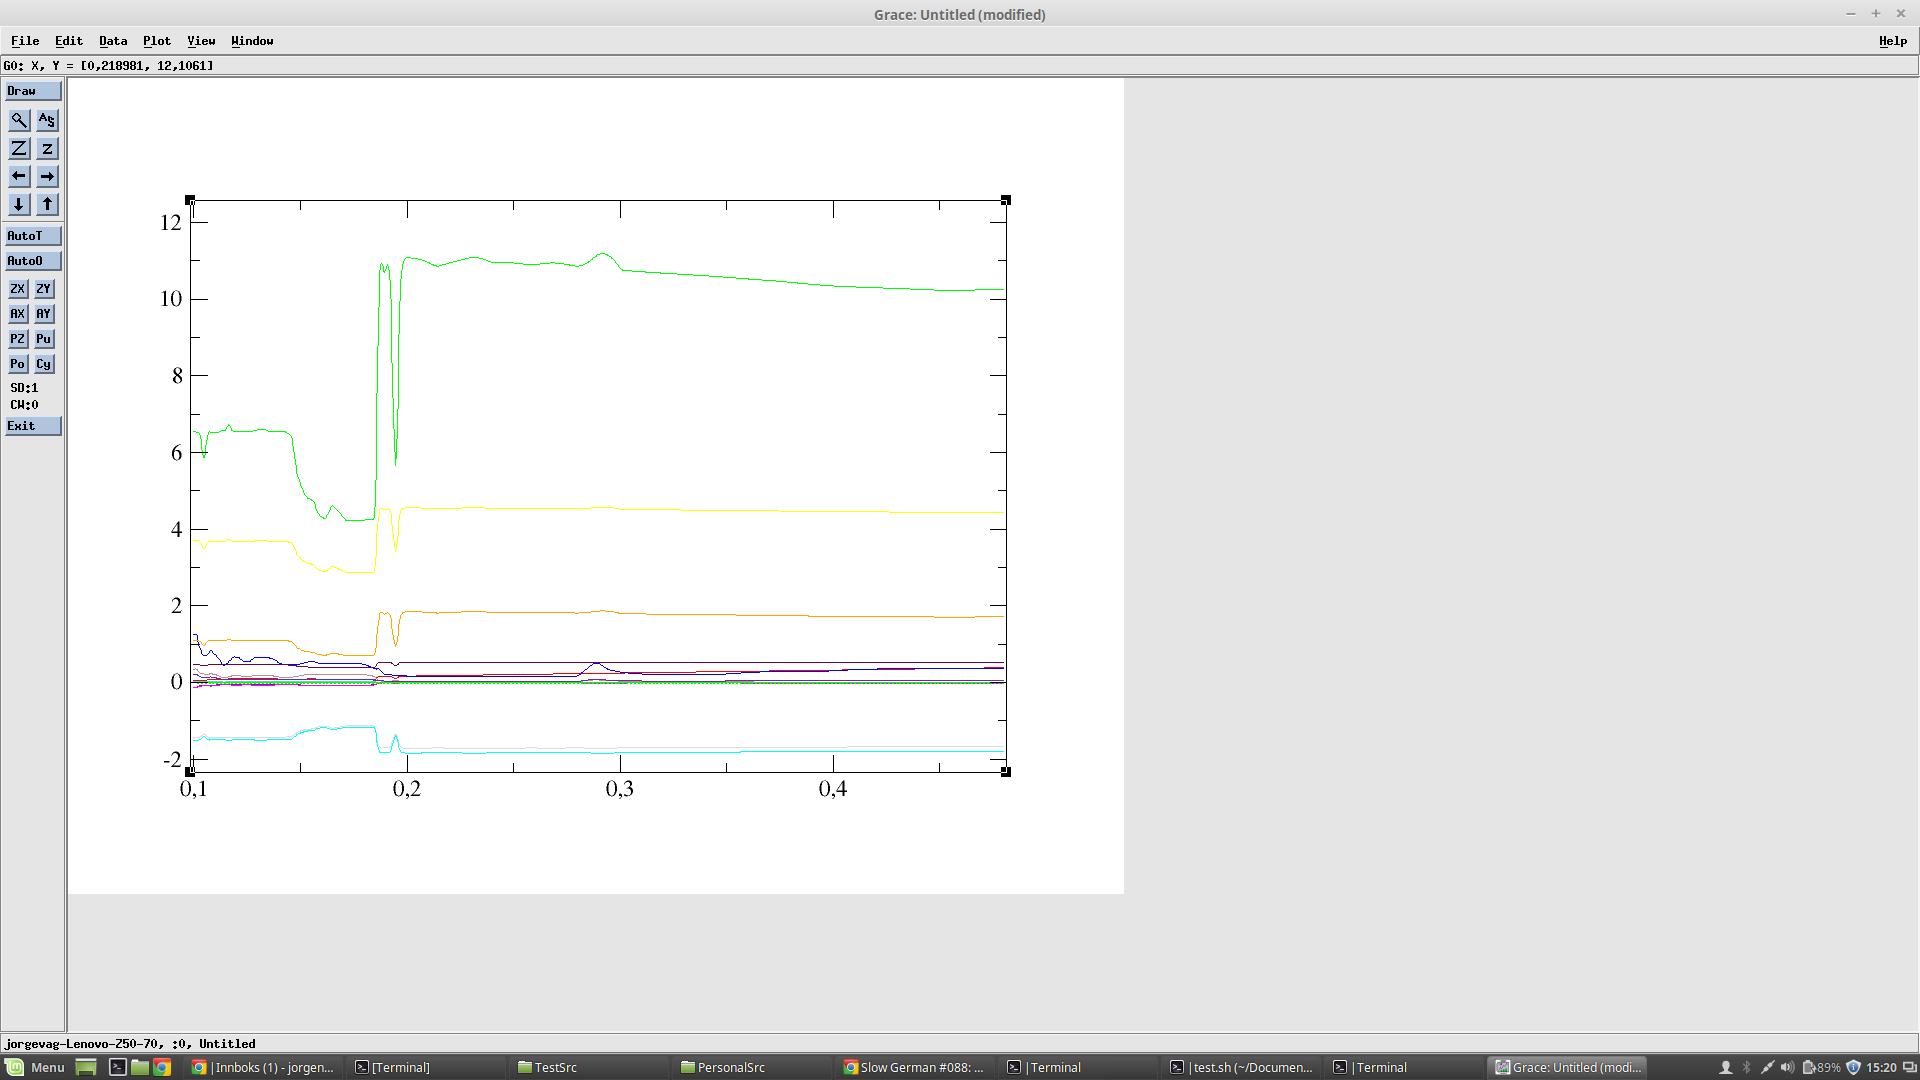
\includegraphics[width=1.0\textwidth]{Figures/result1b.png} 
      \caption{}
      \label{fig2}
      \end{figure}
      %
      \begin{figure}[h!] 
      \centering 
      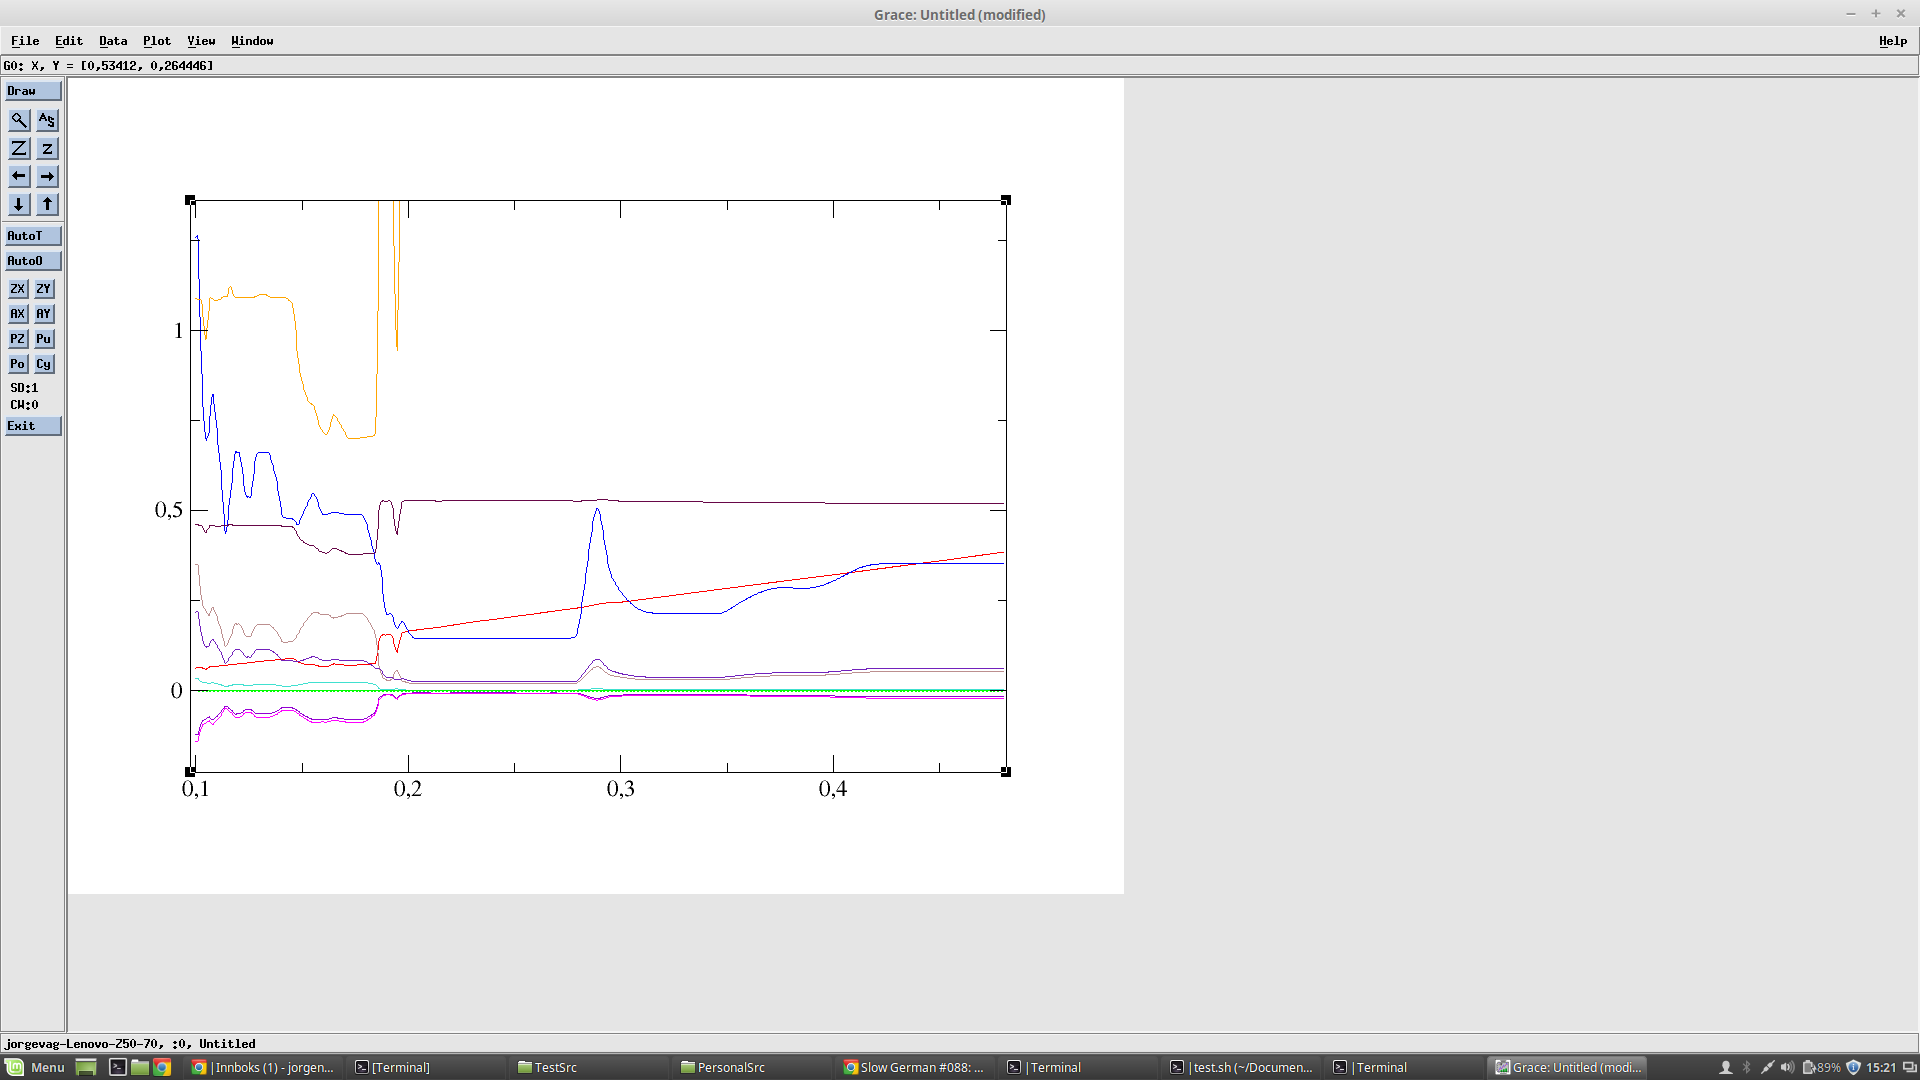
\includegraphics[width=1.0\textwidth]{Figures/result1c.png} 
      \caption{}
      \label{fig3}
      \end{figure}


\end{enumerate}

\section{Spørsmål; Runde 5}
Jeg har prøv å kjøre simuleringer med dataen jeg har for øyeblikket. Resultatene er vist 
lengre nede og ser ikke helt fornuftige ut. Dette dokumentet inneholder derfor
en kjapp gjennomgang av hva jeg har gjort, for å eksludere at jeg ikke har missforstått noe.
All data som er brukt i denne gjennomkjøringen er fra de artiklene du sendte meg tidligere
(til jorgevag@stud.ntnu.no).

\subsection{Data hentet ut fra artiklene}
I figurene 
\ref{fig1E},
\ref{fig2E},
\ref{fig3E},
er grafene funnet i artiklene vist i mot den dataen som faktisk ble hentet ut. I Figur
\ref{fig1E}
er det blandt annet mest overlapp og størst sjanse for feil. Kan også hende at
grafene i den uthentede dataen krysser hverandre feil i de mest overlappede regionene.
\newpage
%
\begin{figure}[h!] 
\centering 
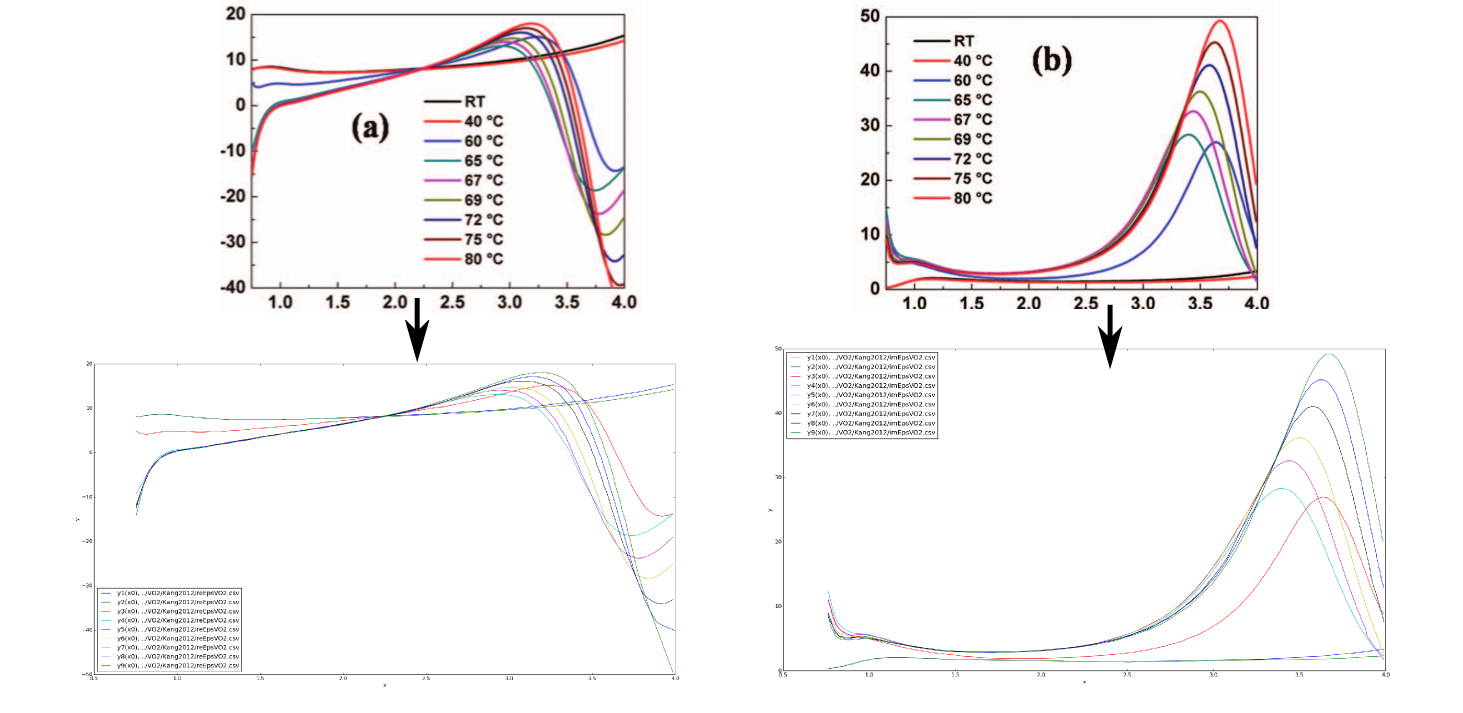
\includegraphics[width=1.0\textwidth]{Figures/KangExtraction.png} 
\caption{Extraction of data from Kang.}
\label{fig1E}
\end{figure}
%
\begin{figure}[h!] 
\centering 
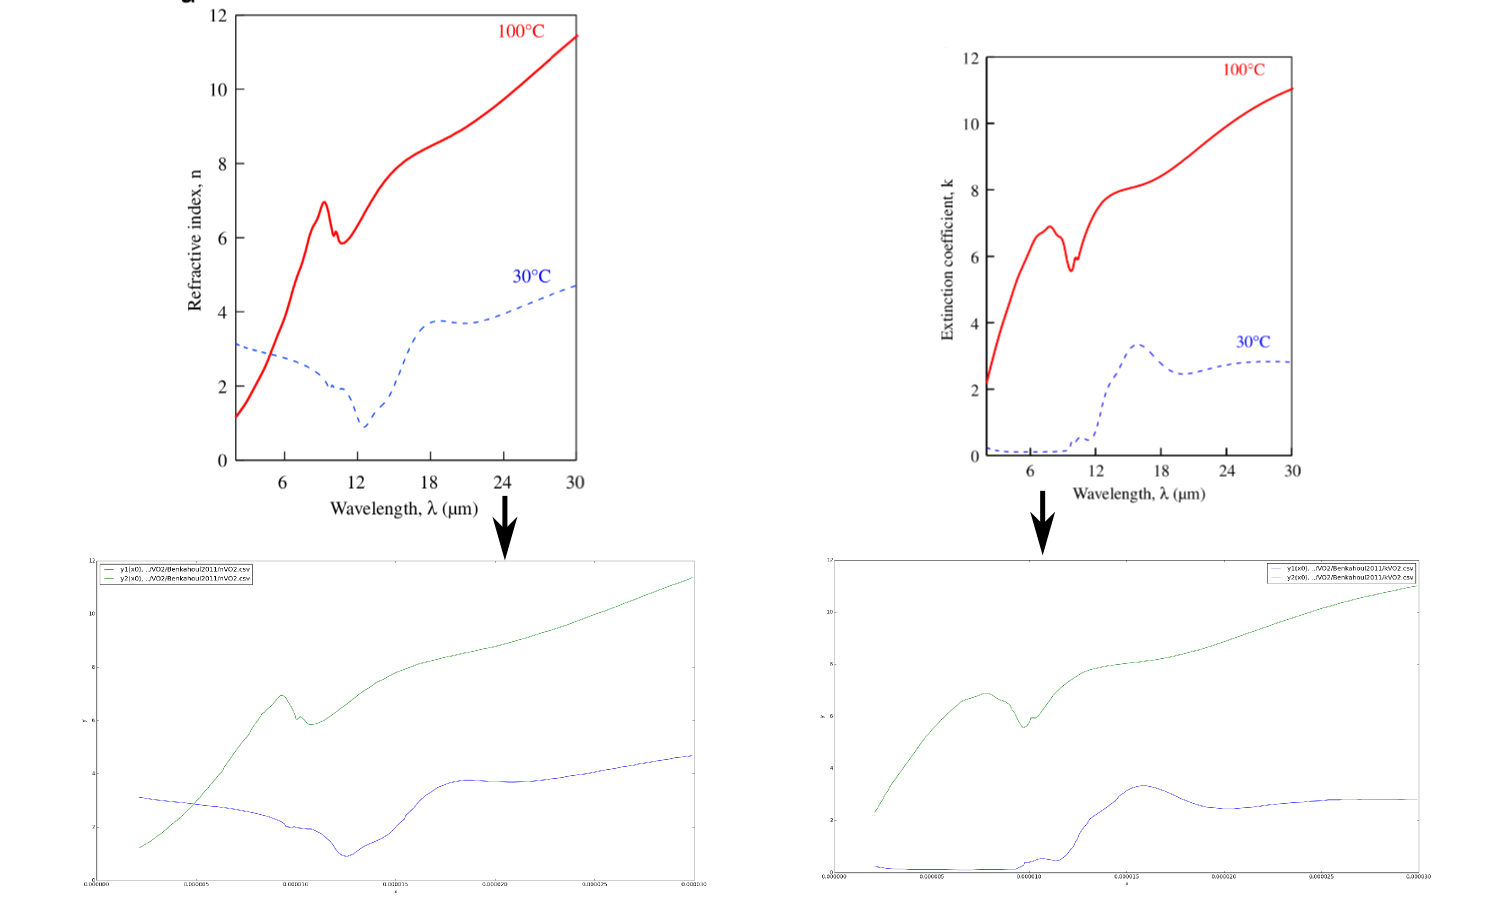
\includegraphics[width=1.0\textwidth]{Figures/BenkahoulExtraction.png} 
\caption{Extraction of data from Benkahoul.}
\label{fig2E}
\end{figure}
%
\begin{figure}[h!] 
\centering 
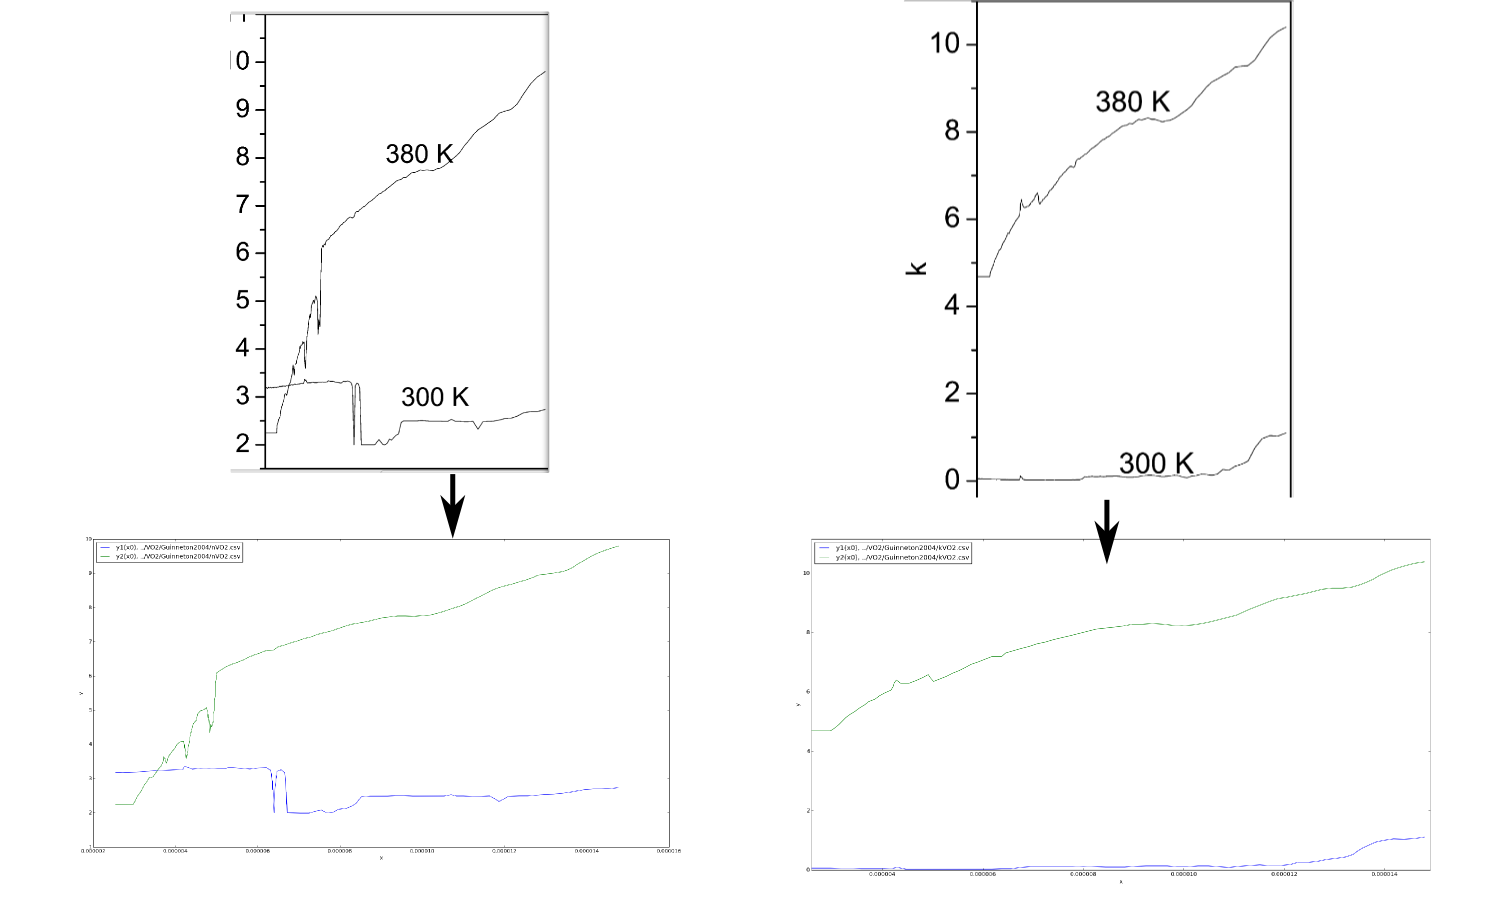
\includegraphics[width=1.0\textwidth]{Figures/GuinnetonExtraction.png} 
\caption{Extraction of data from Guinneton}
\label{fig3E}
\end{figure}
%


\newpage
\subsection{Konvertering av data}
For å konvertere dataen til ekvidistansert n,k-data, brukte jeg samme 
metode som det interpoleringsprogrammet du hjap meg med tidligere. 
Uavhengig om hva enhetene på dataen var, valgte jeg å intrapolere til ekvidistansert
data før jeg konverterte til kompleks brytningsindeks. 
Jeg brukte følgende kode for å konvertere den intrapolerte dataen, som 
her er gitt ved \textbf{re}, \textbf{im} (som kan være permittivitet $\varepsilon$ eller 
brytningsindeks$\hat{n})$:
\begin{lstlisting}[style=FormattedNumber, language=python]
# If the input data is the permittivity/dielectric function, 
# we have to convert to the refractive indicies n,k:
if( isPermittivity ): # data is permittivity
    import scipy.constants
    epsilon0 = scipy.constants.epsilon_0
    # convert from permittivity to refractive index n and absorbtion coeff k:
    absEpsilon = numpy.sqrt( re**2 + im**2)
    n = numpy.sqrt( (absEpsilon + re)/2.0*epsilon0 )
    k = numpy.sqrt( (absEpsilon - re)/2.0*epsilon0 )
else: # the real data should be n, and the imaginary data should be k:
    n = re
    k = im


# convert the x-values to the correct output units: unit=1->x[eV] or unit=2->x[micrometers]
if( unit == 1 ): # eV
    pass # Do nothing
elif(unit == 2): # micrometers
    pass # Do nothing
elif(unit == 3): # nm
    x_min = x_min*(10**(-3))
    x_max = x_max*(10**(-3))
    unit = 2
elif(unit == 4): # m
    x_min = x_min*(10**(6))
    x_max = x_max*(10**(6))
    unit = 2

#write to file
firstLine = str(unit)+'\t'+str(x_min)+'\t'+str(x_max)+'\t'+str(dataPoints)  
numpy.savetxt(ofile, numpy.column_stack((n,k)), delimiter='\t', header=firstLine, comments='')
\end{lstlisting}
For å regne om til n og k, antar jeg at dataen er gitt som $\hat\varepsilon = \hat\varepsilon_r \varepsilon_0$
og bruker:
\begin{align}
   n      &= \sqrt{ \frac{|\hat{\varepsilon}_r| + \varepsilon_r}{2}} 
           = \sqrt{ \frac{|\hat{\varepsilon}| + \varepsilon}{2\varepsilon_0}}\\
   \kappa &= \sqrt{ \frac{|\hat{\varepsilon}_r| - \varepsilon_r}{2}} 
           = \sqrt{ \frac{|\hat{\varepsilon}| - \varepsilon}{2\varepsilon_0}}.
\end{align}

Før jeg leser inn dataen til \textsc{GranFilm}, endrer jeg på 'Energy\_Range' i '.sif'-filen ved å 
lese første linje fra '.nk'-filen. Om verdiene er gitt i $\mu$m (unit=2), konverterer 
jeg med følgende kode (før det skrives inn i '.sif'-filen):
\begin{lstlisting}[style=FormattedNumber, language=python]
# Get 'unit' and energy interval [x1,x2]:
nkfileInfo = nkfileLine1.split()
unit = int(nkfileInfo[0])
x1 = float(nkfileInfo[1])
x2 = float(nkfileInfo[2])

# Check unit:
if( unit == 1 ): # eV
    Emin = x1
    Emax = x2

if( unit == 2 ): # micrometer (wavelength)
    #then convert to eV:
    import scipy.constants as sc
    h = sc.h/sc.e # (planck's constant[J s])/(elementary charge) = planck[eV s]
    c = sc.c # speed of light

    Emin = h*c/( x2*(10**(-6)) )
    Emax = h*c/( x1*(10**(-6)) )
    #ref: http://www.pveducation.org/pvcdrom/properties-of-sunlight/energy-of-photon
\end{lstlisting}
Deretter kjøres \textsc{GranFilm} med'.sif'-filen som input, som igjen kaller tilhørende '.nk'-fil.



\subsection{Test-Simulering}
Dataen nevnt ovenfor ble konvertert til kompleks brytningsindeks og matet inn i GranFilm.
Når all dataen ble simulert (Fig.\ref{figAllD}), så det ut til at den delte seg inn 
i 3 ''regioner'', of jeg frykter dette skyldes ulikheter fra de 3 artiklene.
%
\begin{figure}[h!] 
\centering 
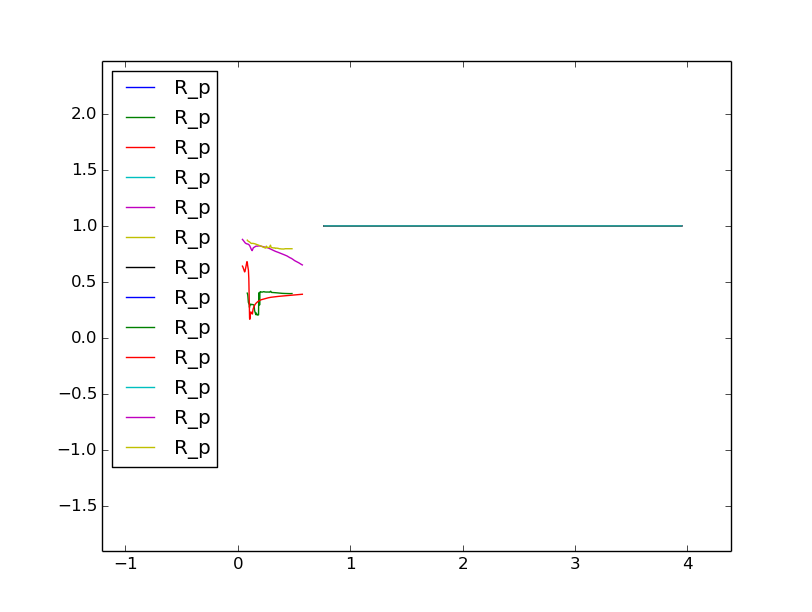
\includegraphics[width=0.5\textwidth]{Figures/vo2RpAll.png} 
\caption{Plot of $R_p = \sqrt{Re(r_p)^2 + Im(r_p)^2}$ for all extracted temperature-data.
Looks like it has formed three different regions shifted from one another.}
\label{figAllD}
\end{figure}
%
%
\begin{figure}[h!] 
\centering 
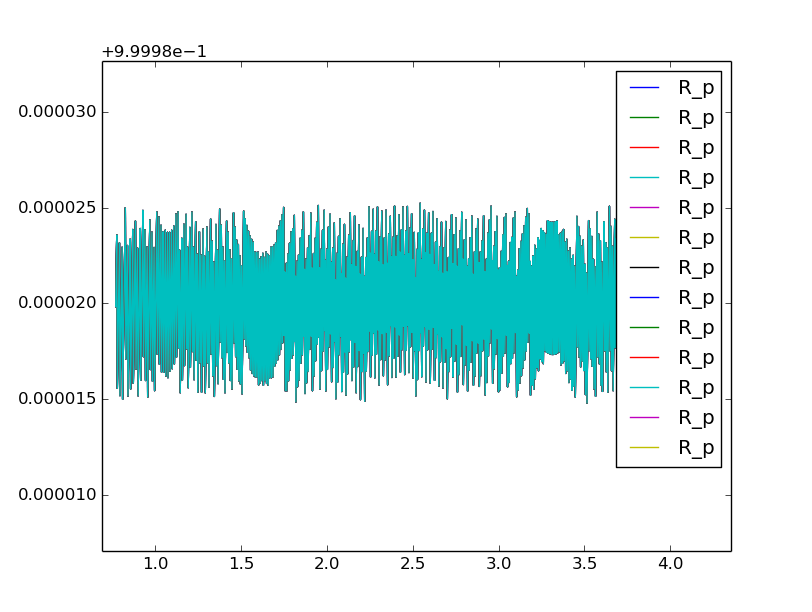
\includegraphics[width=0.5\textwidth]{Figures/kangDataSimulated.png} 
\caption{If I zoom in on the flat part (in $R_p$-plot on previous figure), it looks really messy.}
\label{figAllD1}
\end{figure}
%
En nærmere titt på den flate delen til høyre i Fig.\ref{figAllD}, er vist 
i Fig.\ref{figAllD1}, og jeg får på følelsen av at noe er veldig feil.
Til venstre, Fig. \ref{figAllD2}, ser derimot bedre ut, men vet ikke helt
om resultatet virker fornuftig eller ikke.
%
\begin{figure}[h!] 
\centering 
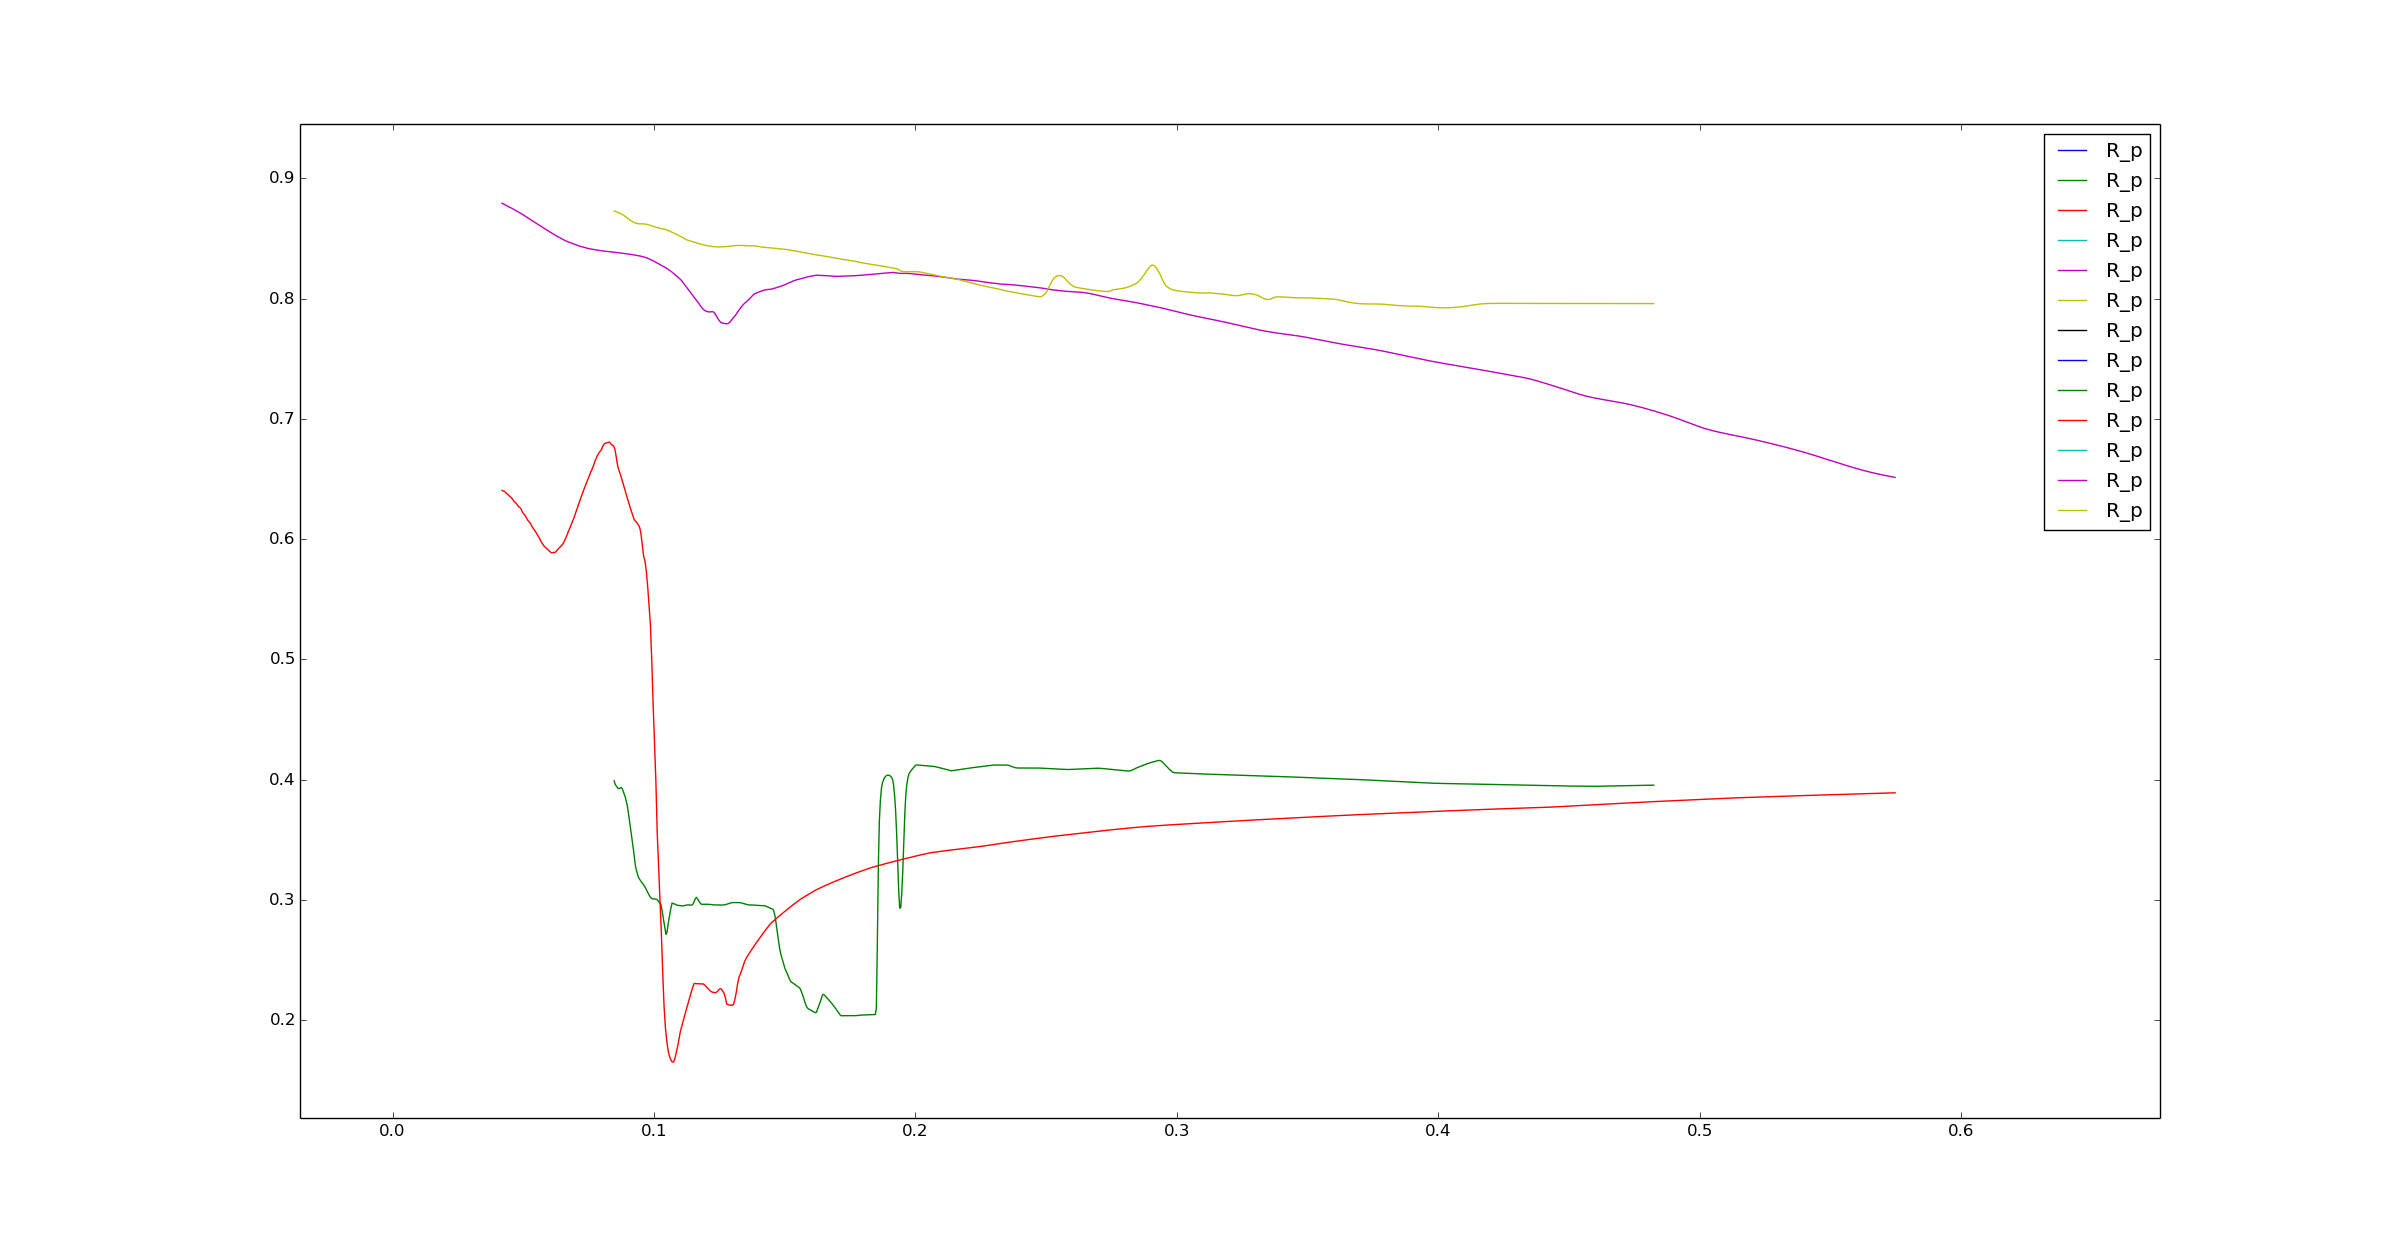
\includegraphics[width=0.5\textwidth]{Figures/niceData.png} 
\caption{The other data in the $R_p$-plot.}
\label{figAllD2}
\end{figure}
%


Sist ble det gjort en simulering for $T = 300$K og $T = 380$K med dataen fra Guinnetion.
Refleksjon og Transmisjon for p-polarizert lys er gitt i Fig.\ref{fig1D} og Fig.\ref{fig2D}.
%
\begin{figure}[h!] 
\centering 
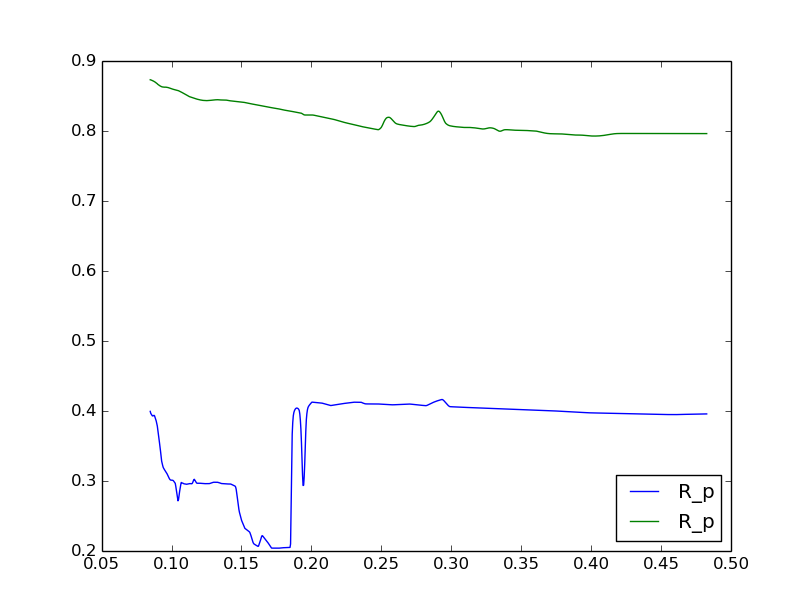
\includegraphics[width=0.5\textwidth]{Figures/vo2Rp_blue300K_green380K.png} 
\caption{ $R_p$ from Guinneton. The blue line is for $T = 300$K; The green line is for $T=380$K.}
\label{fig1D}
\end{figure}
%
%
\begin{figure}[h!] 
\centering 
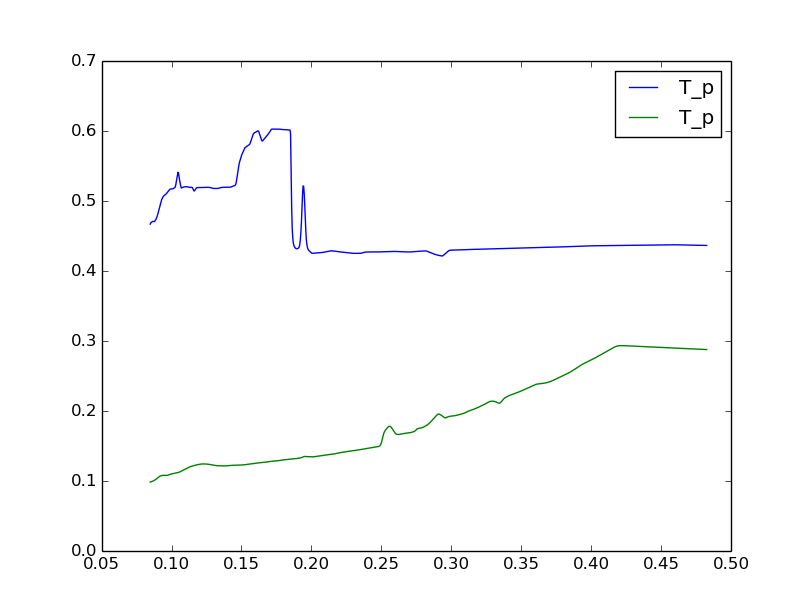
\includegraphics[width=0.5\textwidth]{Figures/vo2Tp_blue300K_green380K.png} 
\caption{ $T_p$ from Guinneton. The blue line is for $T = 300$K; The green line is for $T=380$K.}
\label{fig2D}
\end{figure}
%
\newpage
Jeg er på dette tidspunktet veldig usikker på hvordan jeg finner ut om resultatene er fornuftig eller
feil. Med tanke på hvordan Fig.\ref{figAllD} og Fig.\ref{figAllD1} ser ut, vil jeg uansett anta at 
noe er fryktelig feil. 
\textbf{Er du enig i at dette ser feil ut og har du noen forslag til hva som kan være feil?}


%
\end{document}
